% A.1 Problem
% -----------
\section{Original autofocus implementation}
\label{sec:A.1_title}

Acquisition of in-focus fluorescence microscopy (FM) images comprises an essential aspect of the workflow for integrated array tomography. Focusing the objective lens of the fluorescence microscope can be done manually or by an autofocus routine implemented in the microscope control software, Odemis,\footnote{\href{https://github.com/delmic/odemis}{https://github.com/delmic/odemis}} which performs a dichotomic search for optimal focus (Algorithm \ref{alg:odemis_af}). In this routine an image is recorded at the initial position of the objective lens, after which the lens is translated upwards and downwards by a fixed amount. At each position the focus level is measured by the variance of Laplacian (Algorithm \ref{alg:LAPV}). 

\begin{algorithm}
    \caption{Odemis autofocus routine.}
    \label{alg:odemis_af}
    \begin{algorithmic}
        \While {$s \ge s_{min} \textbf{ and } n < n_{max}$}
        \State $M_{mid} \gets \texttt{acquire\_and\_assess}()$
        \State $z \gets +s$ \Comment{Objective is raised}
        \State $M_{up} \gets \texttt{acquire\_and\_assess}()$
        \State $z \gets  -2s$ \Comment{Objective is lowered}
        \State $M_{dwn} \gets \texttt{acquire\_and\_assess}()$
        \If {$M_{up} == M_{dwn}$} \Comment{Minimized step size reached}
            \State \textbf{break}
        \ElsIf {$M_{up} > M_{mid}$}
            \State $z \gets z_0+s$
        \ElsIf {$M_{dwn} > M_{mid}$}
            \State $z \gets z_0-s$
        \Else \Comment{Best focus found at center}
            \State $z \gets z_0$
            \State $s \gets s/2$ \Comment{Reduce step size by half}
        \EndIf
        \State $n \gets n + 1$
        \EndWhile
    \end{algorithmic}
\end{algorithm}


\begin{algorithm}
    \caption{Variance of Laplacian.}
    \label{alg:LAPV}
    \newsavebox\LAP
    \savebox{\LAP}{$\begin{pmatrix} 1/6 & 2/3 & 1/6 \\ 
                                    2/3 & -10/3 & 2/3 \\
                                    1/6 & 2/3 & 1/6 \end{pmatrix}$}
    \begin{algorithmic}
        \State $L \gets $ \usebox{\LAP} \Comment{Laplacian kernel} \\
        \State $I^{*} \gets \texttt{convolve}(I, L)$ \\
        \vspace{0.2em}
        \Return $\texttt{var}(I^{*})$
    \end{algorithmic}
\end{algorithm}

The objective is vertically translated by a given step size in the direction that increases the focus measure until a decrease is observed. The objective is then iteratively raised and lowered by smaller and smaller increments until a minimum change in the focus measure is reached or the algorithm exceeds the maximum number of attempts. While conceptually sound, it was observed that the autofocus routine is susceptible to errors (Figure \ref{fig:A.1_afruns}), even when executed with seemingly favorable initial conditions (i.e. beginning the routine while in focus). The primary issue is thought to originate from an open loop focus actuator, resulting in objective movements with limited precision. This is evidenced by a significant drop in the focus measure for an image acquired as the objective returns to its starting position (Figure \ref{fig:A.1_afruns}, yellow circle). Photobleaching may also play a role in the decrease of the focus measure.

% --- Fig A.1 (AF runs) ---
\begin{figure}[!tb]
    \centering
    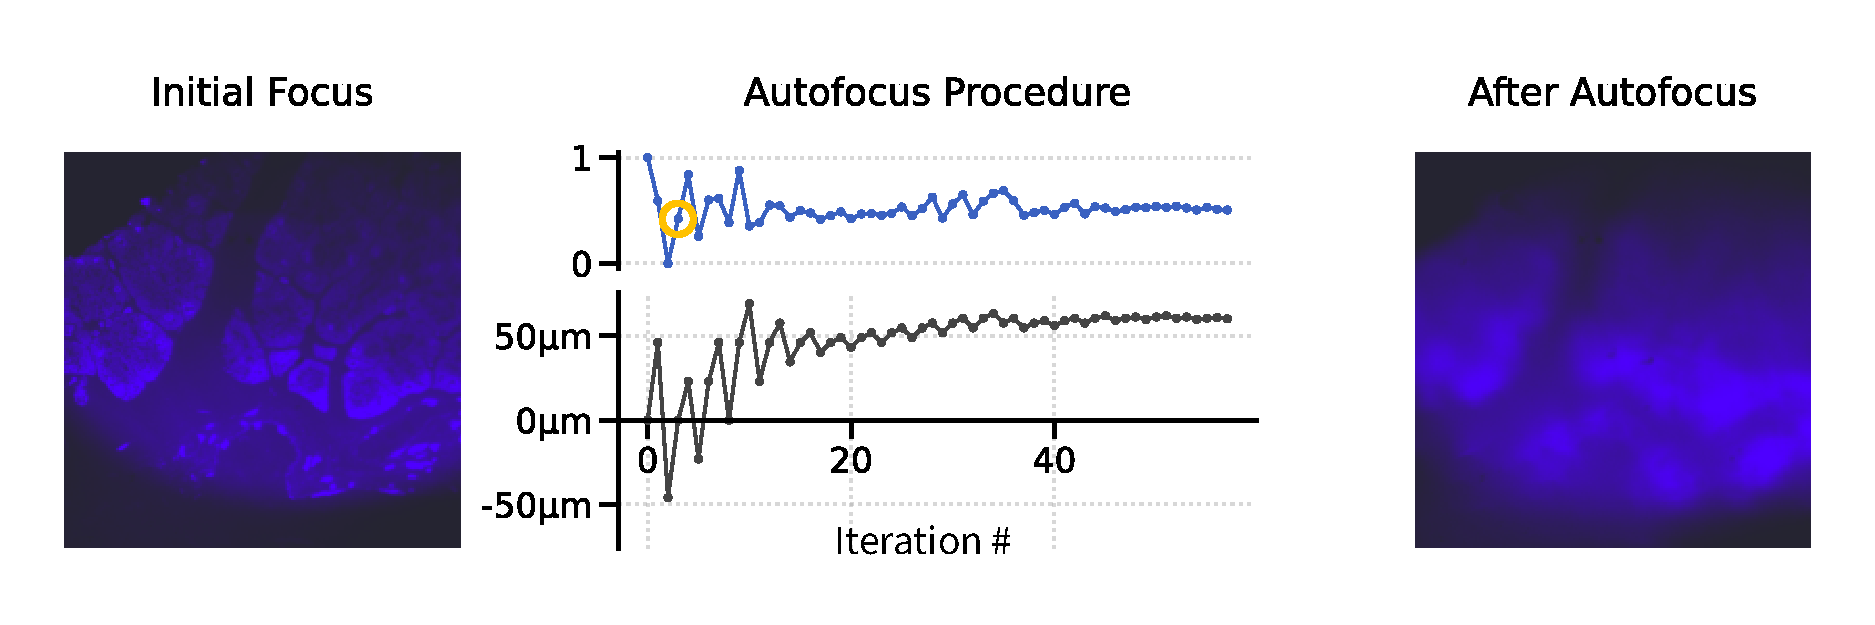
\includegraphics[width=\linewidth]{cppendix-A/figures/figA-1_afruns.pdf}
    \caption{Odemis autofocus routine converging on an out-of-focus image.
    (Left) image from the initial focus position, (center) data from the iterative procedure, (right) image from the final focus position. The two plots show the normalized focus measures (top) and the position of the microscope objective (below) resulting from the dichotomic search. The yellow circle marks the decrease in focus measure when the objective returns to its starting position.}
    \label{fig:A.1_afruns}
\end{figure}


% A.2 Sweeps
% ----------
\section{Analysis of FM focus sweeps}
The results of Figure \ref{fig:A.1_afruns} suggest that a dichotomic search may not be a suitable approach for the autofocus algorithm. Moreover, as will be shown later, Laplacian-based focus measures tend to skew more highly for over-focused images. In order to develop a more robust autofocus algorithm, a series of focus sweeps were conducted over several different $z$ ranges, regions of interest, and fluorescence channels (Figure \ref{fig:A.2_sweeps}). The focus sweeps are analyzed by a selection of different focus metrics (Table \ref{tab:A.1_focus_measures}) compiled from \textcite{pertuz2013analysis}, which examines different focus metrics across a variety of imaging settings and applications. Many of the metrics belong to particular subgroups such as those that involve computing the image gradient (\texttt{GRAE}, \texttt{GRAT}, and \texttt{GRAS}) or the Laplacian (\texttt{LAPE}, \texttt{LAPM}, \texttt{LAPV}, and \texttt{LAPD}). Metrics within each subgroup tend to respond similarly to noise, contrast and window size such that the relative performance depends highly on the particular set of imaging settings \cite{pertuz2013analysis}. The focus metrics were translated from their original Matlab implementation \cite{pertuz2017focus} to Python \cite{Lane_focus-metrics_2022}.

% --- Fig A.2 (sweeps) ---
\begin{figure}[!tb]
    \centering
    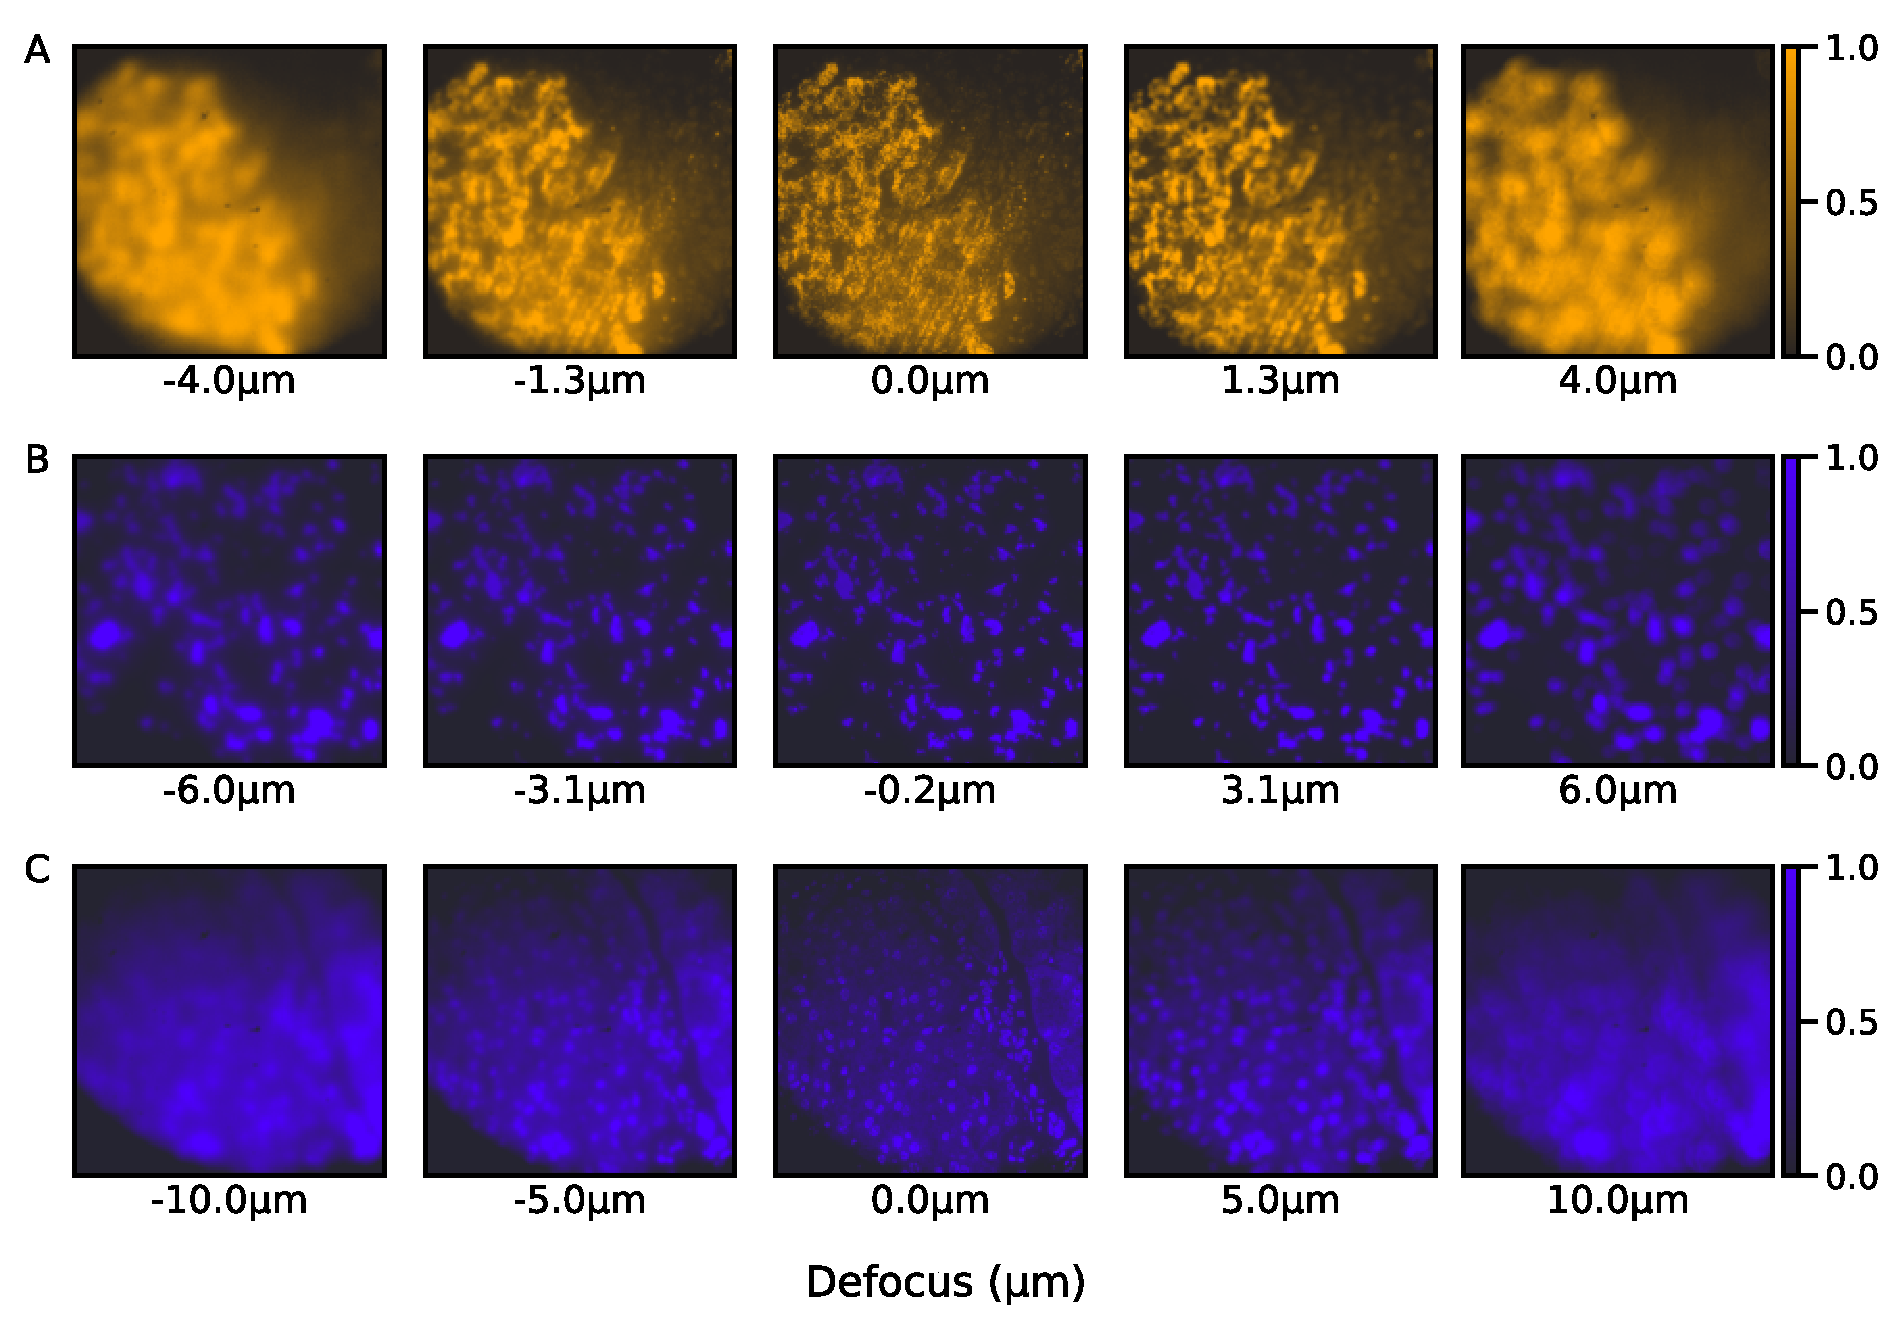
\includegraphics[width=\linewidth]{cppendix-A/figures/figA-2_sweeps.pdf}
    \caption{Sample focus sweeps of the fluorescence microscope.
    (A) An \SI{8}{\micro\meter} sweep over an islet of Langerhans with \SI{555}{\nano\meter} excitation.
    (B) A \SI{12}{\micro\meter} sweep over fluorescent debris on the ITO-coated glass substrate with \SI{405}{\nano\meter} excitation.
    (C) A \SI{20}{\micro\meter} sweep over an islet of Langerhans with \SI{405}{\nano\meter} excitation.}
    \label{fig:A.2_sweeps}
\end{figure}

To assess the relative performance of each focus metric, we perform a consensus analysis to determine how far off each metric is from selecting the correct focus position (Figure \ref{fig:A.3_metrics}). For each focus sweep, the correct focus position is determined by taking the modal value among the 20 focus measures. To better visualize which metrics more frequently return out-of-focus positions, the further away from the modal value a particular curve peaks, the more red that curve appears in the plot. From this analysis it is straightforward to eliminate metrics such as \texttt{ACMO}, \texttt{CURV}, and \texttt{HISE} for which there are multiple red curves. The Laplacian-based metrics can likewise be discarded for their bias towards over-focused images. As expected, there is also a certain degree of redundancy within subgroups. For instance, \texttt{GRAS} (the squared gradient) is virtually equal to \texttt{GRAT} (the thresholded gradient).

% --- Fig A.3 (metrics) ---
\begin{figure}[!tb]
    \centering
    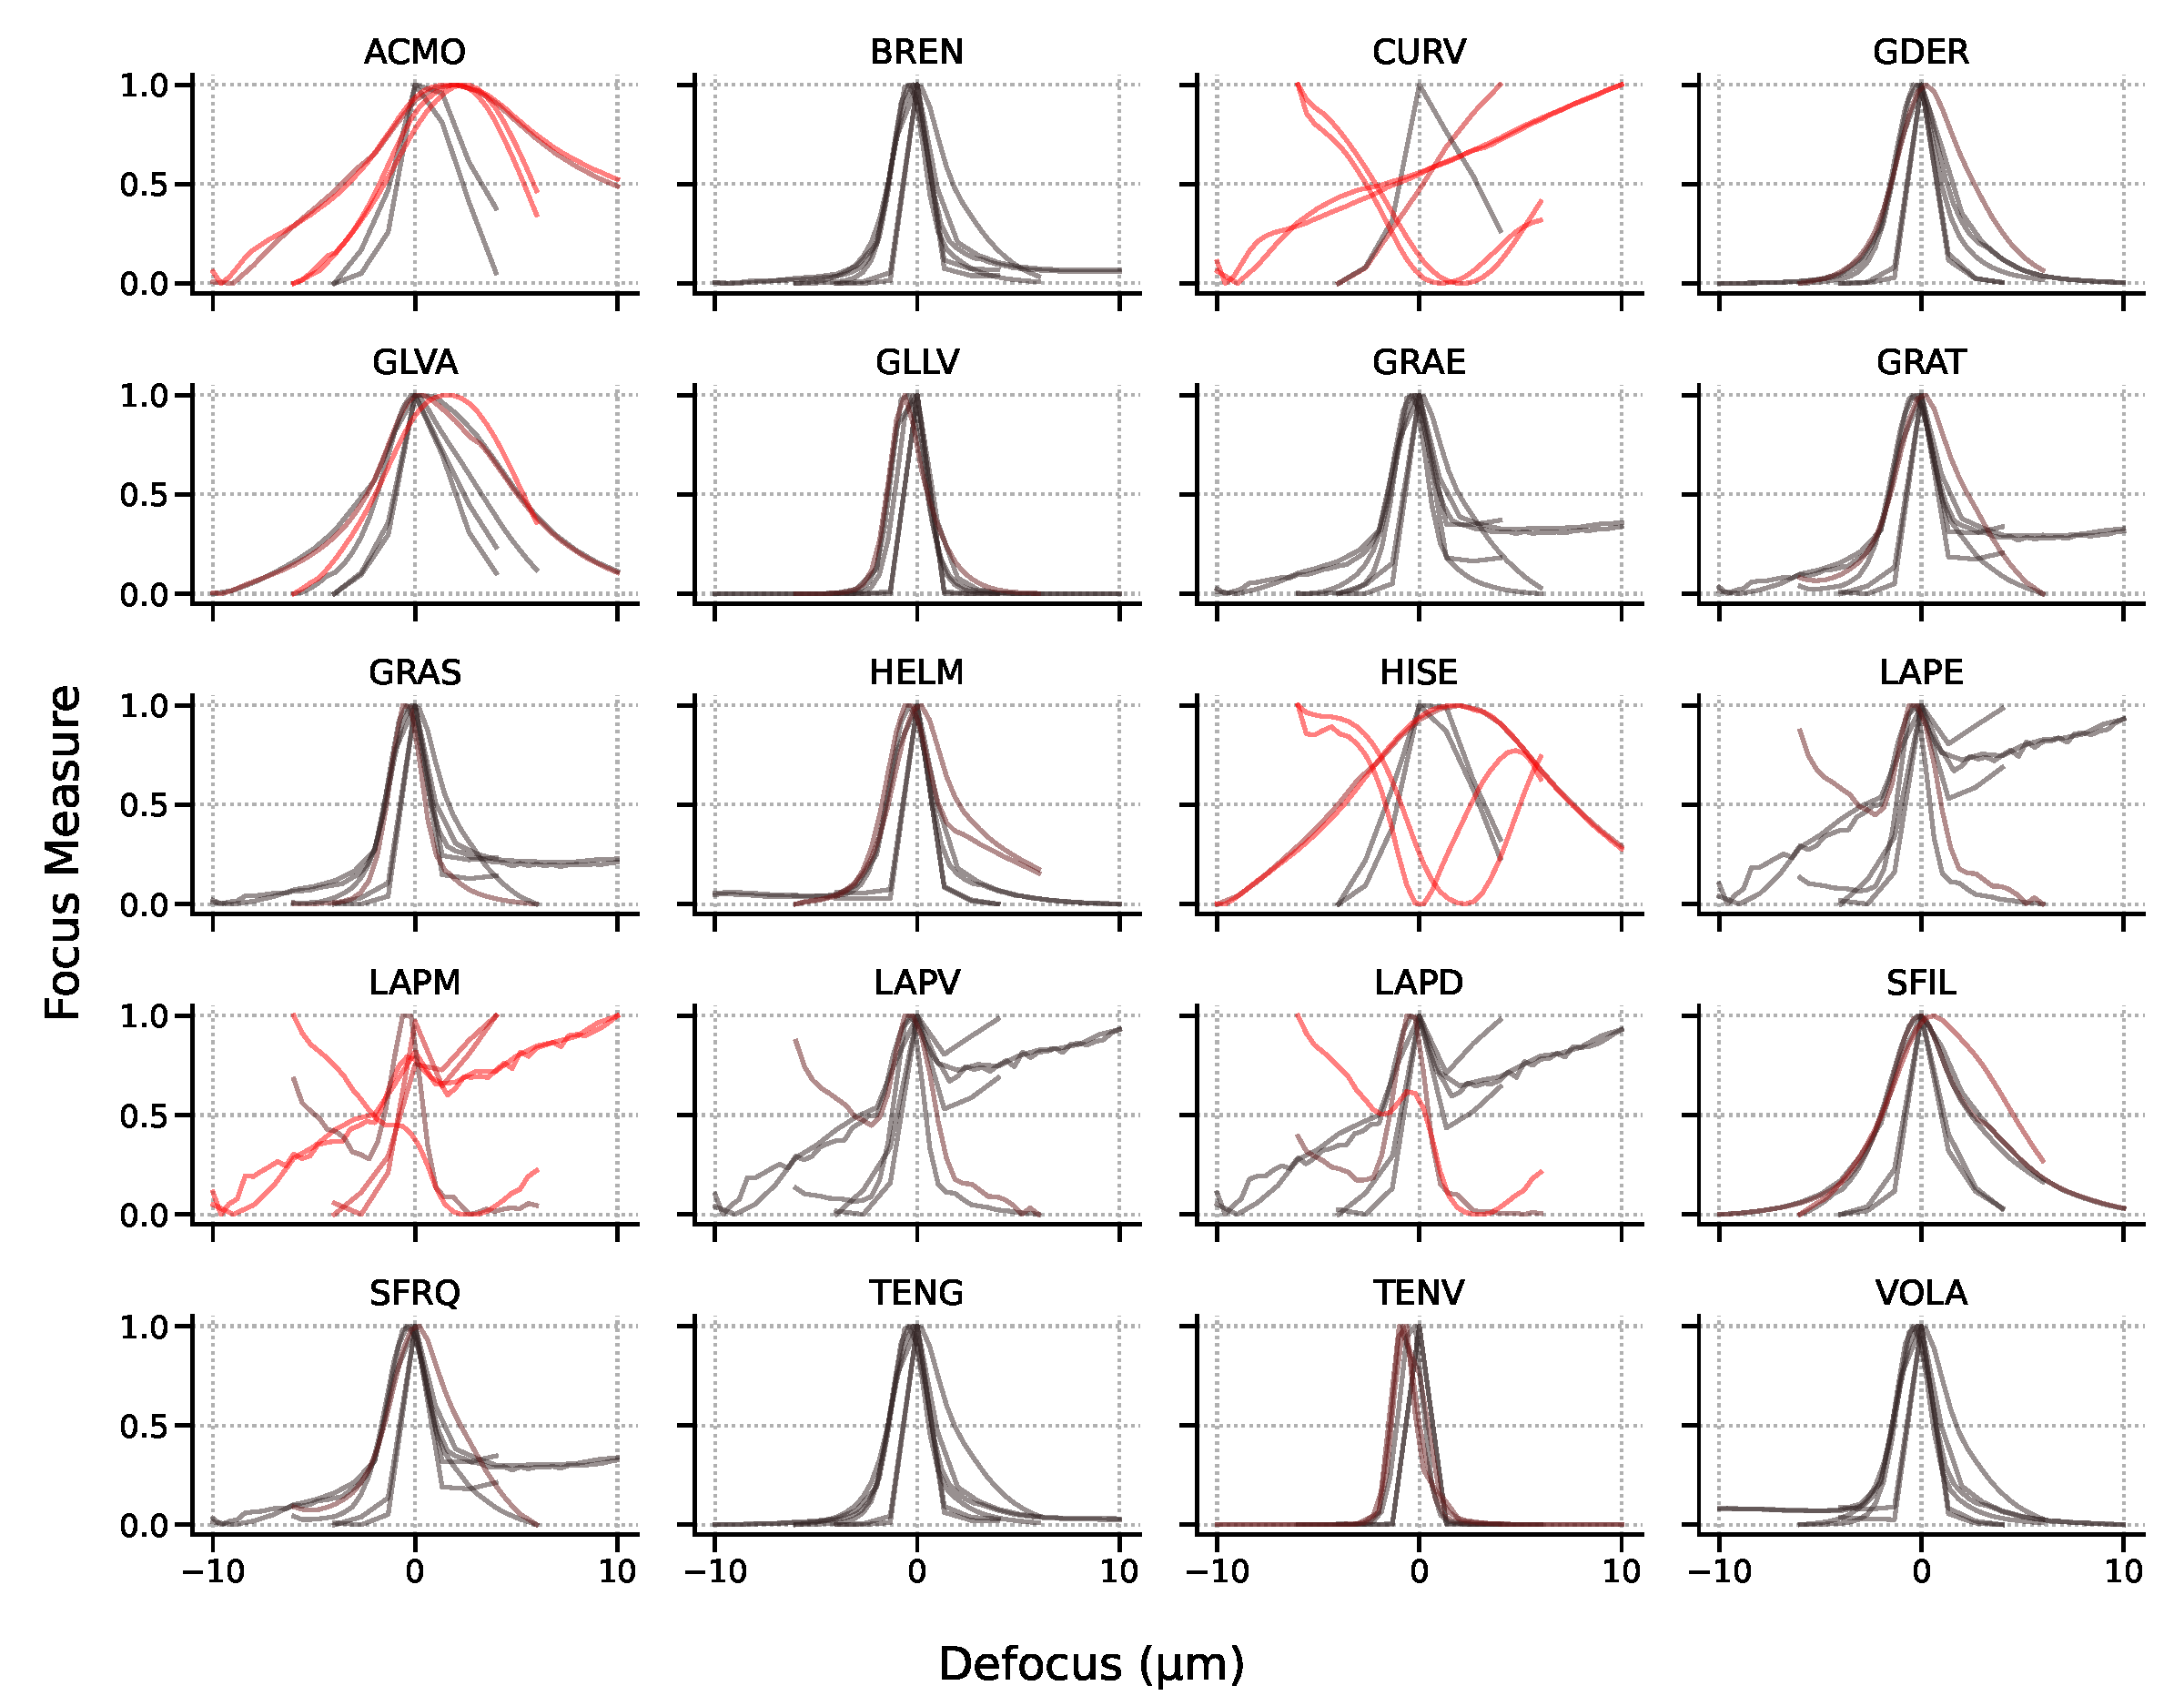
\includegraphics[width=\linewidth]{cppendix-A/figures/figA-3_metrics.pdf}
    \caption{Analysis of 20 potential focus metrics.
    Each subplot shows the focus measures across the six focus sweeps for a particular metric.
    A black color indicates that the peak of the curve is in the consensus (i.e. that the metric returned the correct focus position for that particular sweep).
    Red indicates that the peak of the curve falls outside the consensus, with brighter red signifying that the peak is further away.}
    \label{fig:A.3_metrics}
\end{figure}

After consolidating the candidate focus metrics, we can examine more stringent imaging conditions to explore where the different methods might diverge. To this end, a second round of focus sweeps was recorded in which the images were acquired with decreased exposure times and resolution to present the focus metrics with more challenging settings. The sweeps were then analyzed with the filtered set of candidate focus metrics (Figure \ref{fig:A.4_moresweeps}). The same consensus analysis that was done for the initial set of focus sweeps could not be repeated as the modal value was often erroneous as determined by visual inspection. The correct focus position therefore had to be determined by eye.

% --- Fig A.4 (moresweeps) ---
\begin{figure}[!tb]
    \centering
    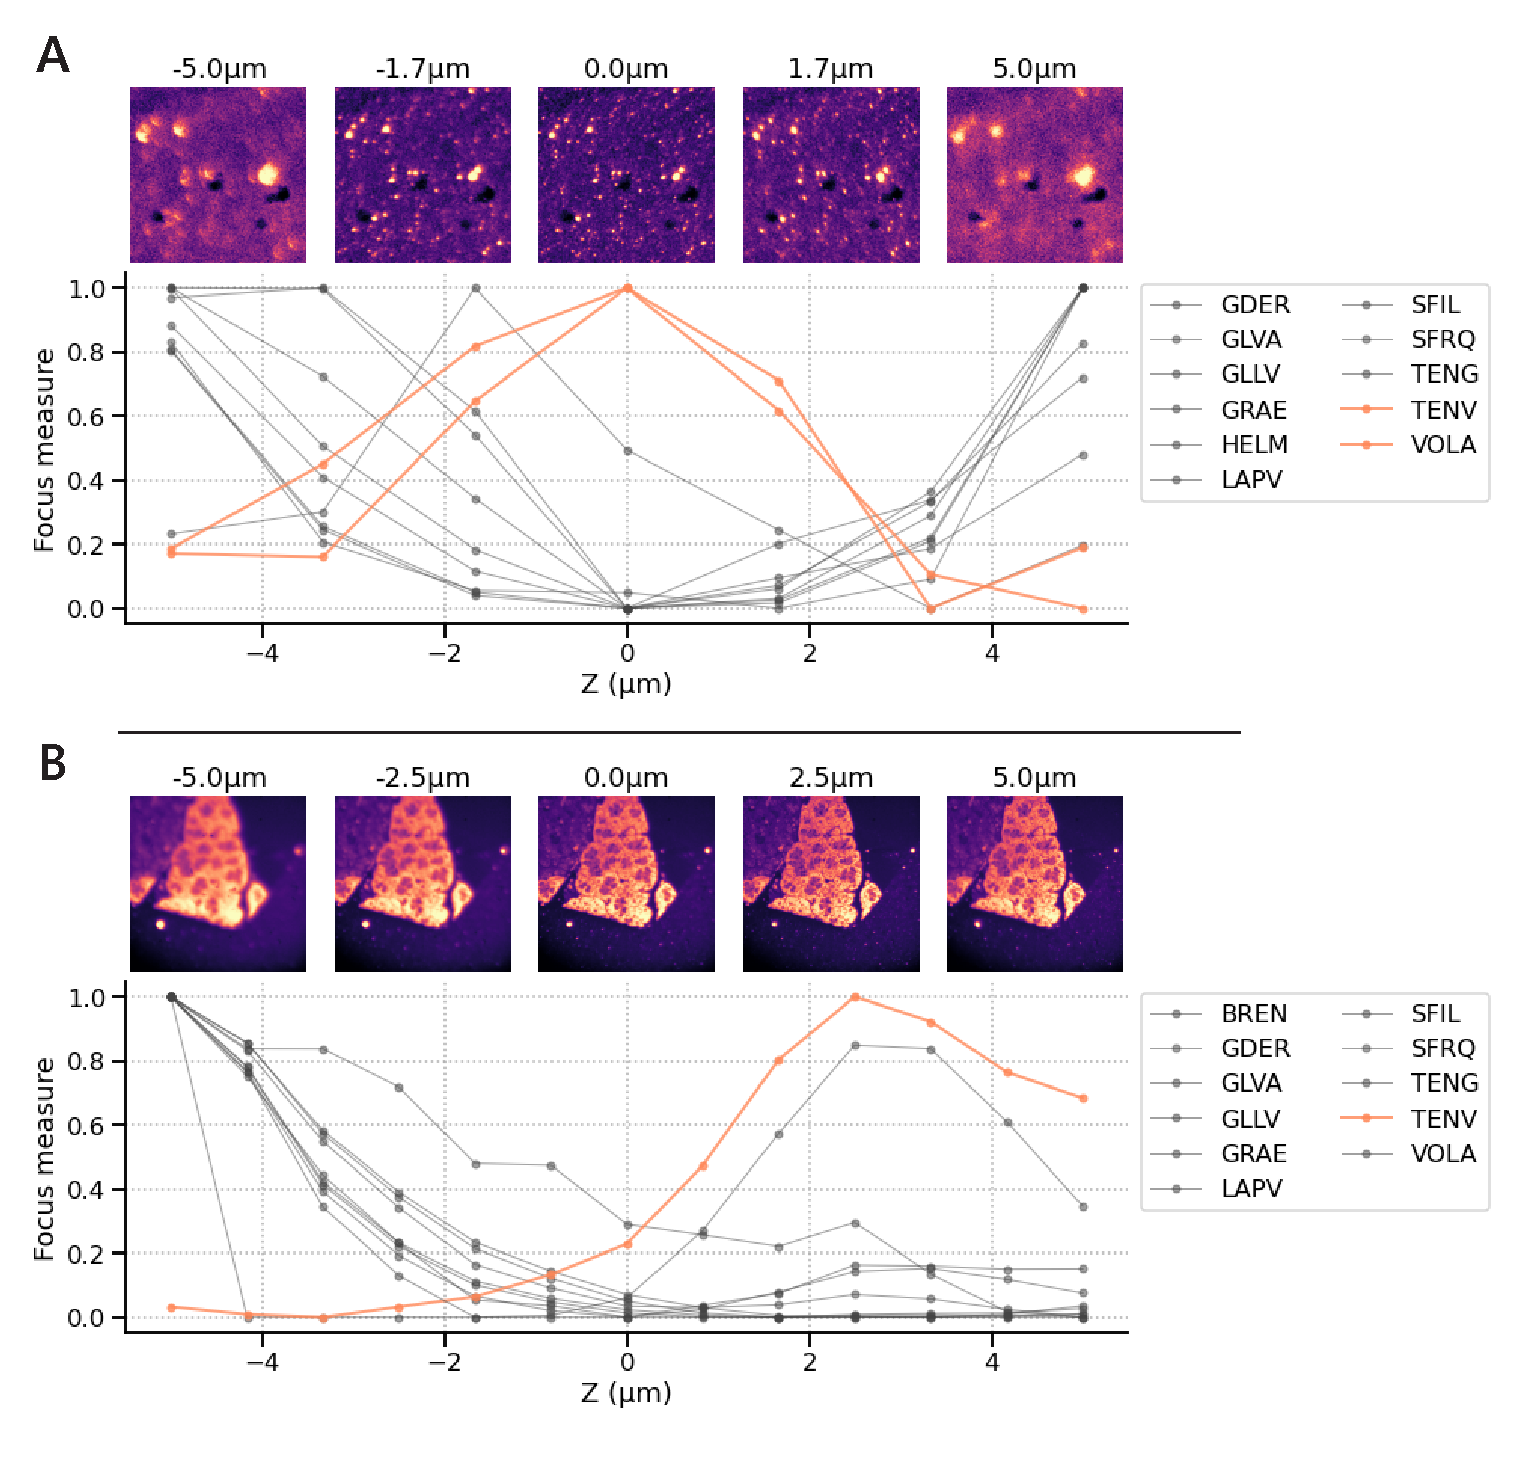
\includegraphics[width=\linewidth]{cppendix-A/figures/figA-4_moresweeps.pdf}
    \caption{Select focus sweeps revealing the robustness of \texttt{TENV} as a focus metric for use with the fluorescence microscope.
    As many of the metrics peaked far from the apparent best focus level, the correct focus position was determined visually.
    (A) A relatively low resolution ($\text{256} \times \text{256}$ \si{\pixel}) focus sweep conducted on the ITO-coated glass background for which only \texttt{TENV} and \texttt{VOLA} yielded the correct focus position.
    (B) A focus sweep acquired on exocrine pancreas tissue with a relatively low exposure time (\SI{100}{\milli\second}) for which only \texttt{TENV} yielded the correct focus position.}
    \label{fig:A.4_moresweeps}
\end{figure}

One metric in particular, \texttt{TENV}, which computes the variance of the image after applying horizontal and vertical Sobel edge detection (Algorithm \ref{alg:TENV}), consistently returned the correct focus position independent of scene, exposure time, and resolution (Figure \ref{fig:A.4_moresweeps}A \& B). A new autofocus routine was therefore developed with \texttt{TENV} as the focus metric and a simple sweep through focus to set the objective position (Algorithm \ref{alg:sweep_af}). To improve precision, the objective position is refined with quadratic interpolation. The new autofocus routine was implemented as an Odemis plugin which could then be integrated into the automated tile acquisitions. Validation was done by automated fluorescence acquisitions on sections of fluorescent HeLa cells embedded in Lowicryl HM20 (Figure \ref{fig:A.5_sections}), resulting in a grid of sharp, well-focused fluorescence images.

% --- Fig A.5 (sections) ---
\begin{figure}[!tb]
    \centering
    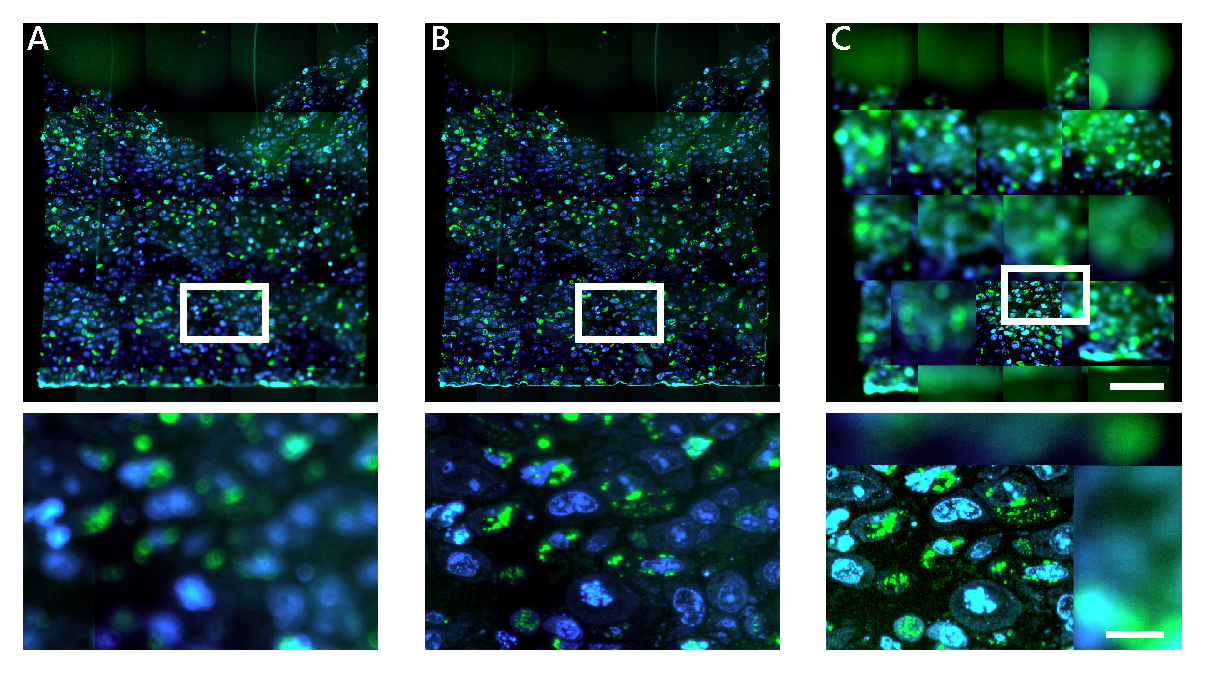
\includegraphics[width=\linewidth]{cppendix-A/figures/figA-5_sections.pdf}
    \caption{Autofocus routine based on focus sweeps and \texttt{TENV} yields best results for automated fluorescence imaging.
    (A) no autofocus routine, (B) the autofocus routine described here, and (C) the default autofocus routine implemented in Odemis.
    All automated fluorescence acquisitions were conducted on the same section of fluorescent HeLa cells.
    Scale bars: (A\,--\,C) \SI{100}{\micro\meter}; (insets) \SI{20}{\micro\meter}.}
    \label{fig:A.5_sections}
\end{figure}


%
\begin{algorithm}
    \caption{Tenengrad variance.}
    \label{alg:TENV}
    \newsavebox\sobelh
    \savebox{\sobelh}{$\begin{pmatrix} 1 &  2 &  1 \\ 
                                       0 &  0 &  0 \\
                                      -1 & -2 & -1 \end{pmatrix}$}
    \newsavebox\sobelv
    \savebox{\sobelv}{$\begin{pmatrix} 1 & 0 & -1 \\ 
                                       2 & 0 & -2 \\
                                       1 & 0 & -1 \end{pmatrix}$}
    \begin{algorithmic}
        \State $S_H \gets $ \usebox{\sobelh} \Comment{Horizontal Sobel filter} \\
        \State $S_V \gets $ \usebox{\sobelv} \Comment{Vertical Sobel filter} \\
        \vspace{0.5em}
        \State $I^{*}_H \gets \texttt{convolve}(I, S_H)$ \\
        \vspace{-1em}
        \State $I^{*}_V \gets \texttt{convolve}(I, S_V)$ \\
        \vspace{0.5em}
        \Return $\texttt{var}\left((I^{*}_H)^2 + (I^{*}_V)^2\right)$
    \end{algorithmic}
\end{algorithm}
%

%
\begin{algorithm}
    \caption{Autofocus algorithm based on sweep through focus.}
    \label{alg:sweep_af}
    \begin{algorithmic}
        \State $M_{max} = 0$
        \State $z \gets -\Delta z/2$
        \For {$i \textbf{ in range } N$}
            \State $M \gets \texttt{acquire\_and\_assess}()$
            \State $M_{max} = \textbf{max}(M, \,M_{max})$
            \State $z \gets +\Delta z/N$
        \EndFor
        \State $z \gets \texttt{QIFFT}([M_{max - 1}, \,M_{max}, \,M_{max + 1}])$ \Comment{Quadratic interpolation}
    \end{algorithmic}
\end{algorithm}
%




 % --- Table A.1 (references) ---
\begin{table}[!tbh]
    \centering
    \caption{Reference list for focus metrics.}
    \label{tab:A.1_focus_measures}
    \begin{tabular}{@{}llr@{}}
    \toprule
    & Focus metric & Reference \\
    \arrayrulecolor{black!30}\midrule
    \texttt{ACMO} & Absolute central moment & \cite{shirvaikar2004optimal} \\
    \texttt{BREN} & Brenner's focus measure & \cite{santos1997evaluation} \\
    \texttt{CURV} & Image curvature & \cite{helmli2001adaptive} \\
    \texttt{GDER} & Gaussian derivative & \cite{geusebroek2000robust} \\
    \texttt{GLVA} & Gray-level variance & \cite{krotkov1986range} \\
    \texttt{GLVV} & Gray-level local variance & \cite{pech2000diatom} \\
    \texttt{GRAE} & Energy of gradient & \cite{subbarao1992focusing} \\
    \texttt{GRAT} & Thresholded gradient & \cite{santos1997evaluation} \\
    \texttt{GRAS} & Squared gradient & \cite{eskicioglu1995image} \\
    \texttt{HELM} & Helmli's measure & \cite{helmli2001adaptive} \\
    \texttt{HISE} & Histogram entropy & \cite{krotkov1986range} \\
    \texttt{LAPE} & Energy of Laplacian & \cite{subbarao1992focusing} \\
    \texttt{LAPM} & Modified Laplacian & \cite{nayar1990shape} \\
    \texttt{LAPV} & Variance of Laplacian & \cite{pech2000diatom} \\
    \texttt{LAPD} & Diagonal Laplacian & \cite{thelen2008improvements}  \\
    \texttt{SFIL} & Steerable filters-based & \cite{minhas20093d} \\
    \texttt{SFRQ} & Spatial frequency & \cite{eskicioglu1995image} \\
    \texttt{TENG} & Tenegrad & \cite{krotkov1986range} \\
    \texttt{TENV} & Tenengrad variance & \cite{pech2000diatom} \\
    \texttt{VOLA} & Vollat's correlation-based & \cite{santos1997evaluation} \\
    \arrayrulecolor{black}\bottomrule
    \end{tabular}
\end{table}


% --- Fig A.6 (timing) ---
\begin{figure}[!tb]
    \centering
    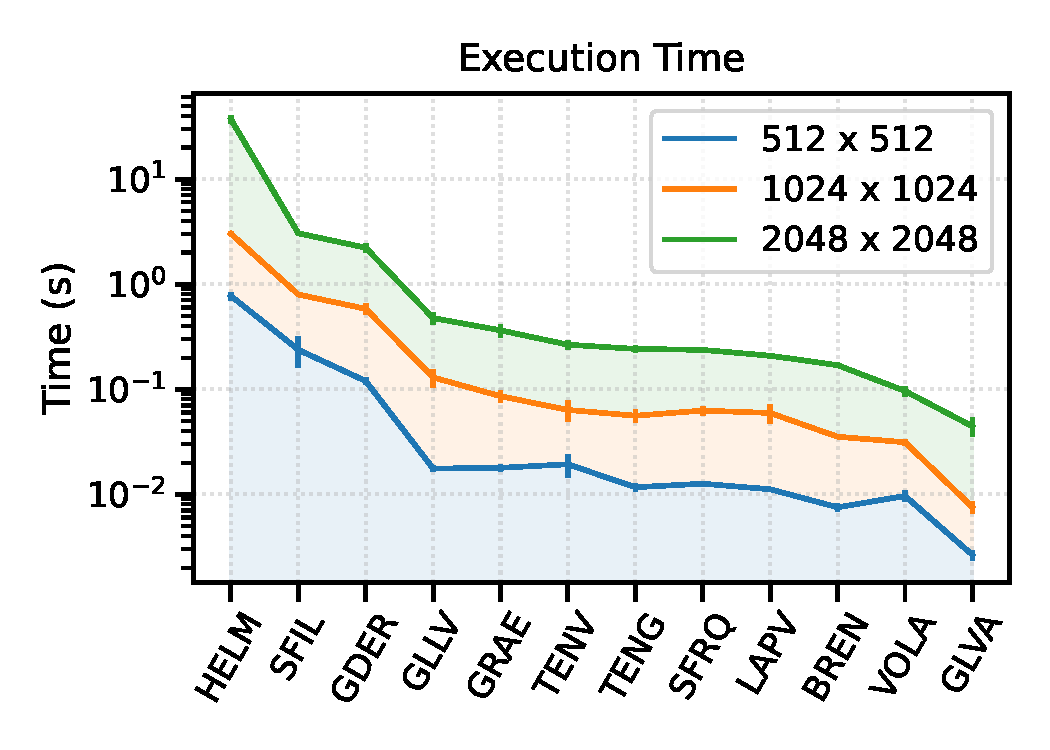
\includegraphics[width=0.7\linewidth]{cppendix-A/figures/figA-6_timing.pdf}
    \caption{Execution times for the filtered set of candidate focus metrics.
    $\text{512}\times\text{512}$, $\text{1024}\times\text{1024}$, and $\text{2048}\times\text{2048}$ denote the image dimensions.}
    \label{fig:A.6_timing}
\end{figure}
